%%==========================
%% chapter01.tex for SJTU Master Thesis
%% based on CASthesis
%% modified by wei.jianwen@gmail.com
%% version: 0.3a
%% Encoding: UTF-8
%% last update: Dec 5th, 2010
%%==================================================

%\bibliographystyle{sjtu2} %[此处用于每章都生产参考文献]
\chapter{数据库驱动认知无线电的相关标准}
\label{chap:standard}

认知无线电网络作为一种最有前景的频谱资源稀缺问题的解决方案,目前还没有在实际中大规模部署,而数据库驱动认知无线电网络也正处于研究阶段,其标准化工作也在进行中。本节我们对Internet工程任务组(Internet Enginering Task Force, IETF)针对数据库驱动认知无线电网络制定的标准做一概述。

IETF近期发布了白空间数据库接入协议PAWS(Protocol to Access White-Space)的Internet草案\cite{zhu2014protocol}。
部分已经分配的频谱可以在不产生干扰的情况下供认知用户使用,这部分频谱资源称为白空间(White Space)。对白空间的利用可以大大提高无线频谱资源的使用率。数据库驱动认知无线电网络通过地理信息数据库来实现设备间的频谱共享,取代了原来设备必须通过频谱感知来决定可用频谱的过程。
地理信息数据库能够跟踪可用频谱并对用户设备提供这些信息。这种方式将实现复杂度和频谱策略的限制由终端设备转移到地理信息数据库上来,简化了频谱策略变化引起的麻烦,使得系统在升级时只需要改变数据库的相应策略而不用改变大量的终端设备,提供了更好的可扩展性。它可以方便地集成一些参数,包括地理位置和时间等,来为频谱共享和频谱管理提供改进的空间。在未来,还可能考虑集成其他参数例如用户优先级、信号类型、功率等。

为提供上述服务,数据库需要记录和更新必要的信息来保护主用户,这些信息可能包括地理位置、天线高度、传输功率、操作时间等。对于数据库必须遵守的一些规则集,例如获得和更新主用户保护信息的日程,主用户保护规则等,可以根据管理域的不同而变化,这些不同的规则集只要求数据库能够处理,对认知用户来讲不需要知道其中的细节。

网络中的认知用户分为主设备和从设备。主设备不同于主用户,主设备属于认知用户,能够使用预先建立的Internet连接通过PAWS协议从数据库获得可用频谱信息。从设备只能通过主设备间接获得可用频谱信息。一个简单的数据库驱动认知无线电网络如图\ref{fig:db-cr}所示。


\begin{figure}[!htp]\label{fig:db-cr}
  \centering
  \includegraphics[width=0.8\textwidth]{figures/chap3/db-cr}\bicaption[fig:db-cr]{数据库驱动认知无线电网络示意图}{数据库驱动认知无线电网络示意图}{Fig}{Illustration of Database-driven CRNs}
\end{figure}


由于主设备和从设备工作过程相似,区别只在于主设备从数据库获取可用频谱信息而从设备从主设备获取可用频谱信息,因此,在本文的后续部分,所有提到的认知用户即指主设备。数据库驱动认知无线电网络的典型工作步骤为:

(1)认知用户获取相应数据库的统一资源标识符(Uniform Resource Identifier,URI)信息。统一资源标识符可以在认知用户上静态地配置,也可以通过其他方式动态地获取。

(2)认知用户与数据库之间建立HTTPS会话。

(3)认知用户选择性地向数据库发送初始化信息。如果数据库收到认知用户的初始化信息,则回应一个初始化响应消息。

(4)数据库可以要求认知用户在请求服务之前注册到数据库。

(5)认知用户向数据库提交可用频谱请求消息。

(6)数据库向认知用户发送响应消息,内容包含可用频谱信息。

(7)认知用户可以向数据库发送频谱使用的通知消息。

(8)如果数据库收到频谱使用通知消息,它将回应一个确认消息。


具体地讲,PAWS协议包括如下几个功能模块:数据库发现、初始化、设备注册、可用频谱查询、频谱使用通知。下面简要对这几个功能模块进行介绍。

\begin{enumerate}
\item 数据库发现:

认知用户可以预先静态地配置一个或多个数据库的URI以便查询。此外,也可以采用动态的方式来获取数据库URI,即在认知用户端静态指定一个列表服务器,然后通过列表服务器的查询服务动态地获得可用频谱信息。如果数据库URI发生变化,静态配置方式需要修改URI,而列表服务器方式只需要更改列表服务器的配置而无需终端做任何修改。


\item 初始化:

一旦认知用户启动,它必须启动初始化进程来与数据库交互一些必要的信息,数据库需要告知认知用户其规则集中的参数值,例如阈值距离、持续时间等。初始化过程如图\ref{fig:initialization}所示。

\begin{figure}[!htp]\label{fig:initialization}
  \centering
  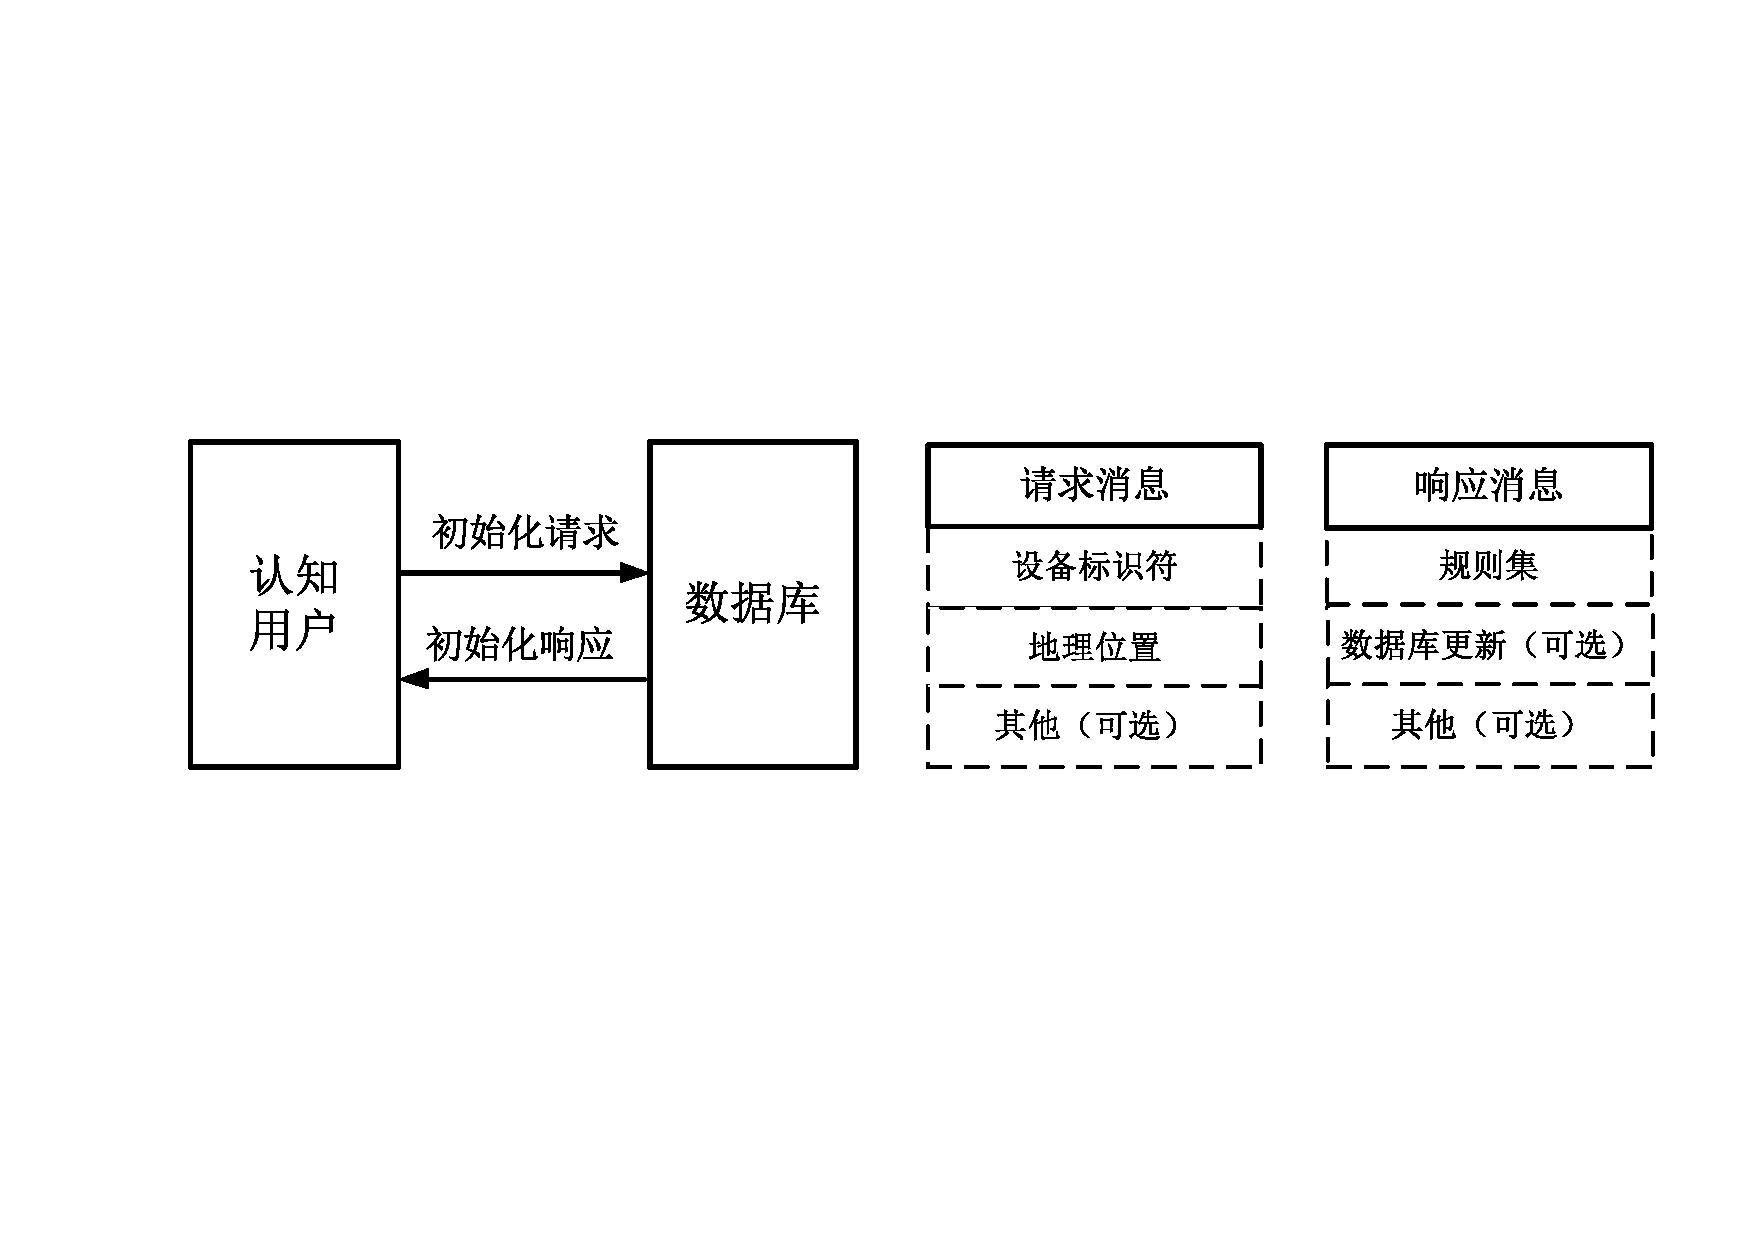
\includegraphics[width=0.8\textwidth]{figures/chap3/standard/initialization}\bicaption[fig:initialization]{用户初始化过程}{用户初始化过程}{Fig}{Process of Initialization}
\end{figure}

设备标识符是用户身份的唯一标识,规则集是指数据库管辖范围内约定的通信规则。数据库更新字段用于在数据库更改URI时通知认知用户进行相应更改。

\item 设备注册:

有些规则集要求认知用户向数据库发送注册信息以设定某些操作参数,例如FCC规定固定用户必须将其设备所有者和操作者以及设备标识符、地理位置、天线高度等信息上报给数据库。数据库可以要求认知用户以独立的请求方式进行注册,也可以允许认知用户将注册消息作为可用频谱查询消息的子集发送给数据库。用户注册过程如图\ref{fig:registration}所示。

\begin{figure}[!htp]\label{fig:registration}
  \centering
  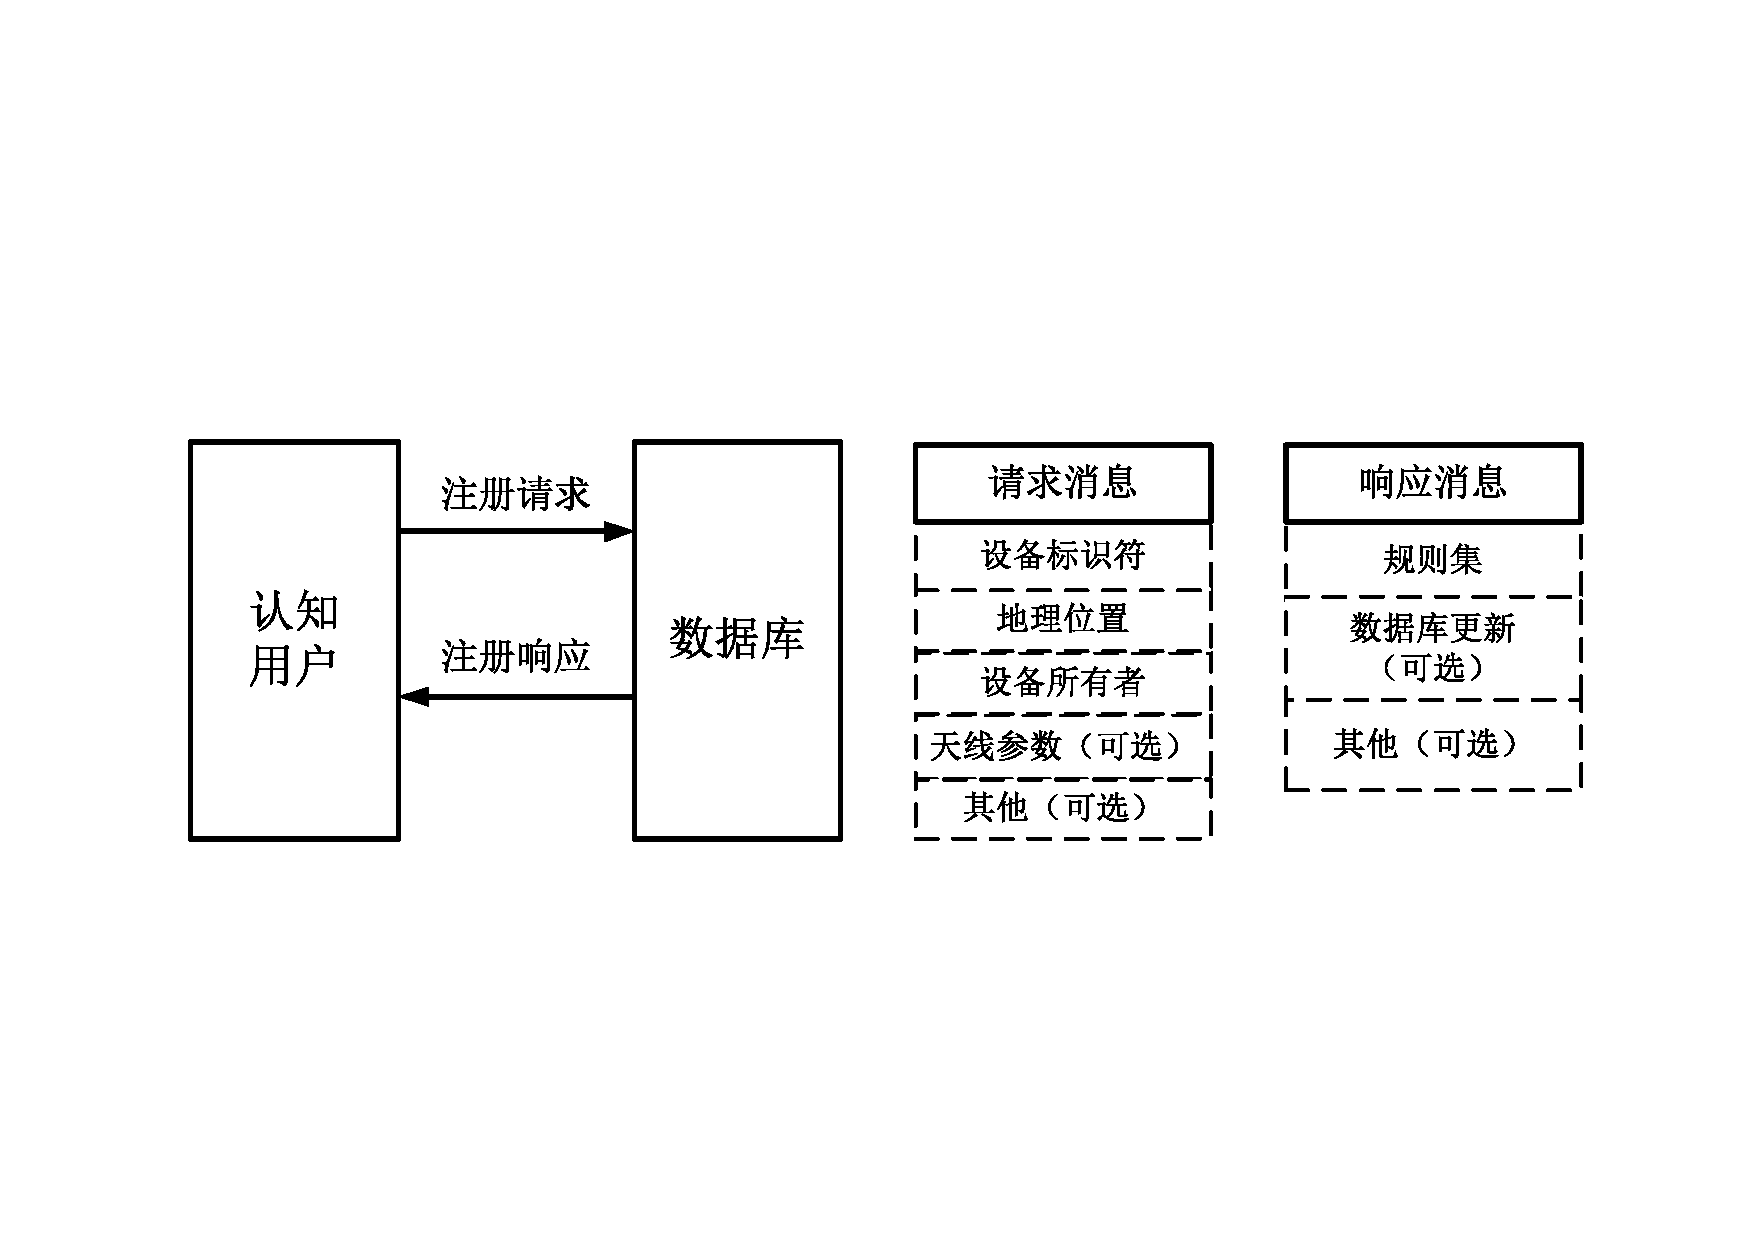
\includegraphics[width=0.8\textwidth]{figures/chap3/standard/registration}\bicaption[fig:registration]{用户注册过程}{用户注册过程}{Fig}{Process of Registration}
\end{figure}

设备所有者信息包含所有者的唯一身份标识。天线参数主要包括天线高度、天线类型、天线方向、天线辐射辐射类型、天线增益以及天线极化方式等信息。

\item 可用频谱查询及通知:

为从数据库获得可用频谱信息,认知用户发送查询消息,根据其地理位置和必须的参数请求可用频谱。数据库根据请求消息中的地理位置将该位置的可用频谱信息告知认知用户。认知用户在可用的频谱列表中进行选择并可以将频谱使用信息上报给数据库。可用频谱查询及通知过程如图\ref{fig:query}所示。

\begin{figure}[!htp]\label{fig:query}
  \centering
  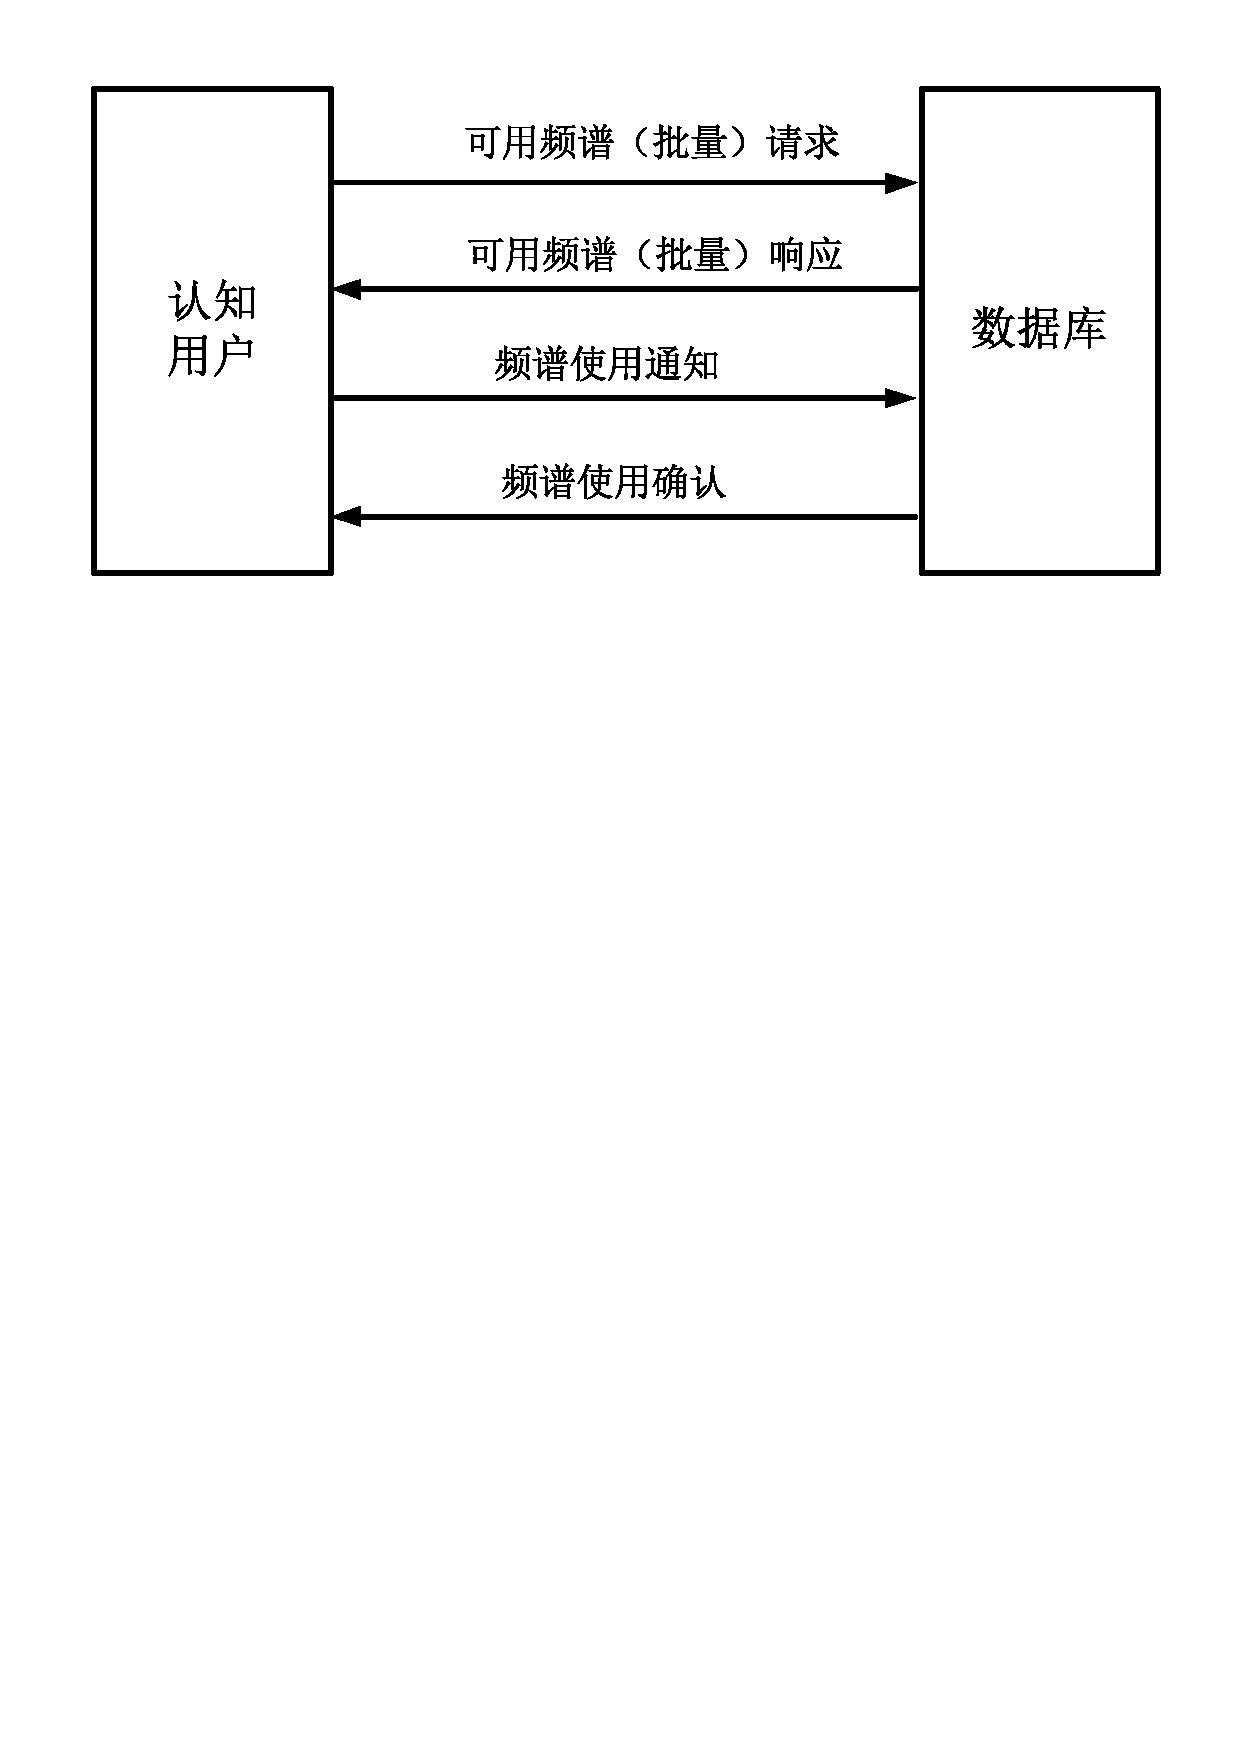
\includegraphics[width=0.6\textwidth]{figures/chap3/standard/query}\bicaption[fig:query]{可用频谱查询过程}{可用频谱查询过程}{Fig}{Process of Availability Spectrum Query}
\end{figure}

其中查询及响应内容如图\ref{fig:query-1}所示。

\begin{figure}[!htp]\label{fig:query-1}
  \centering
  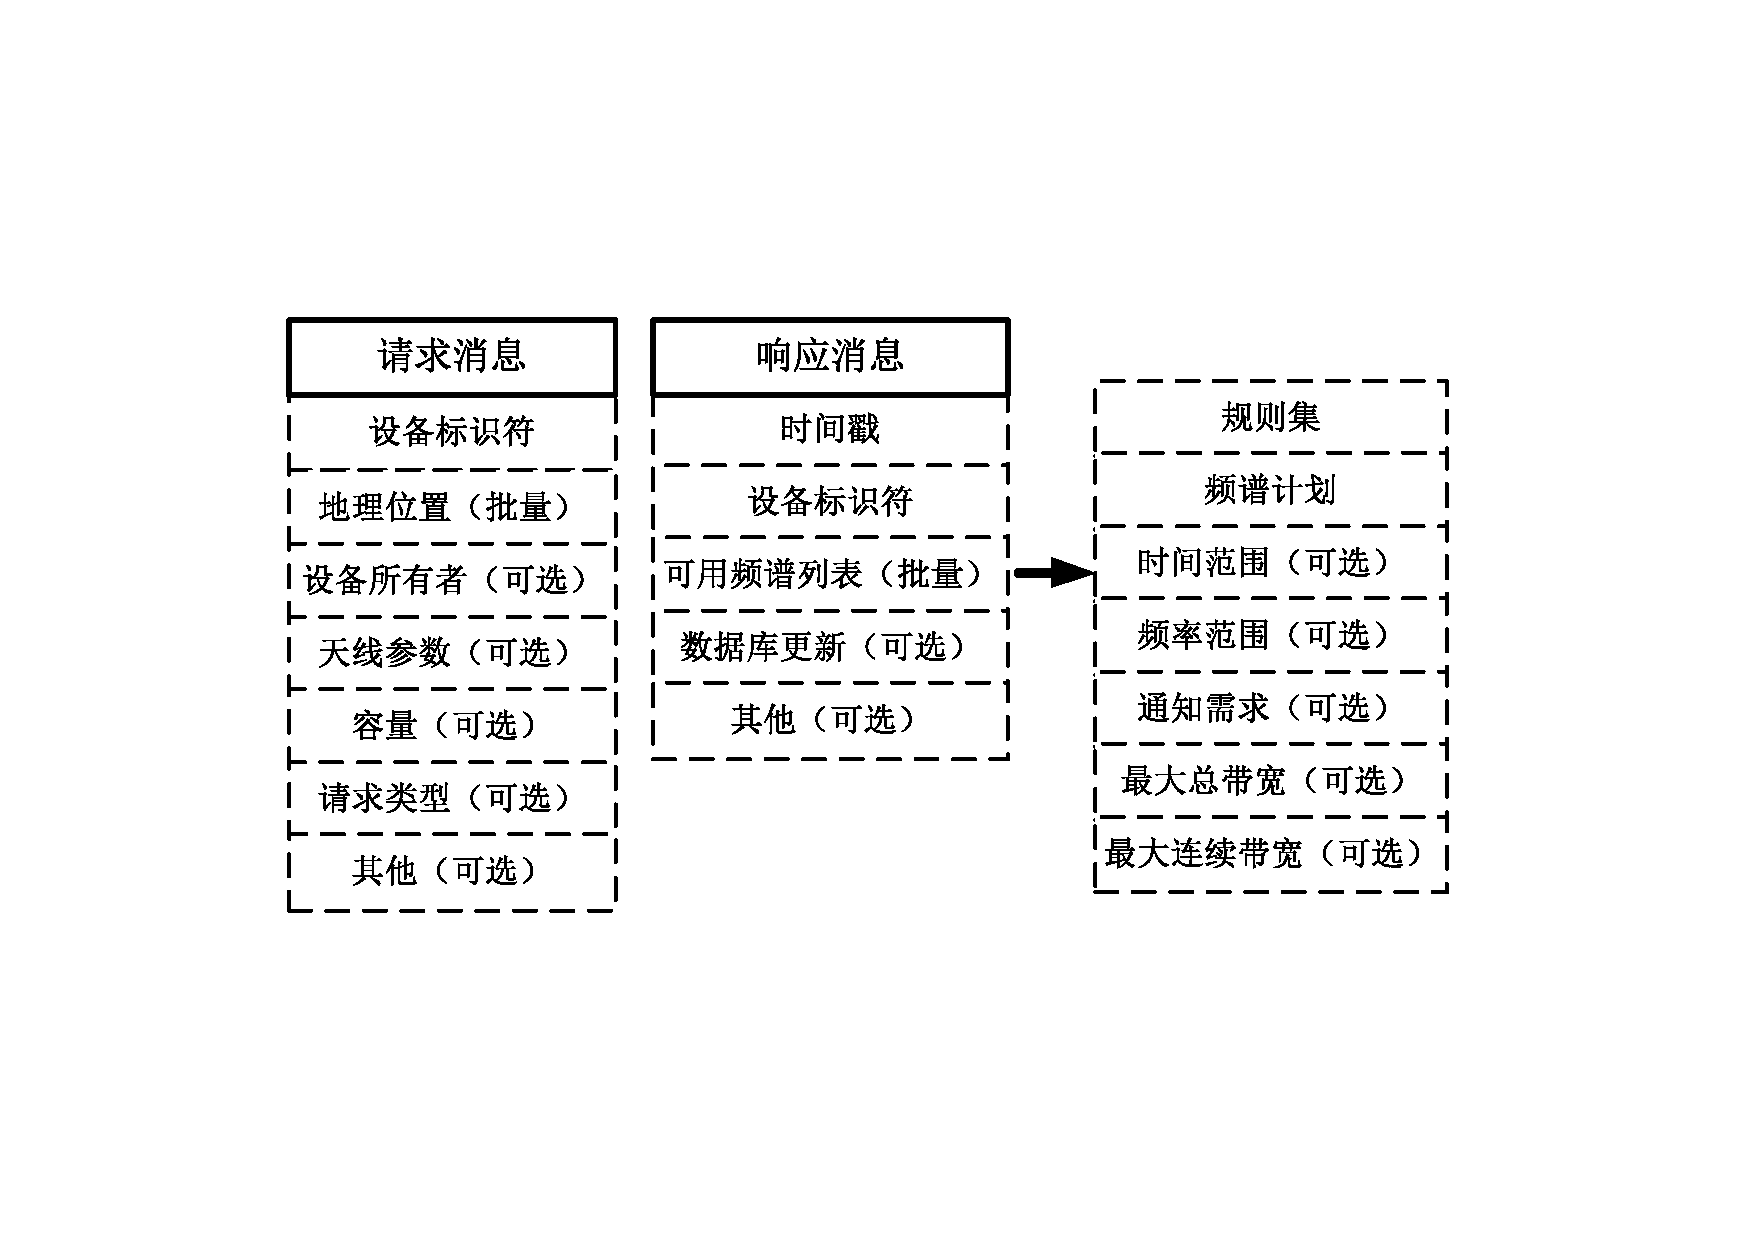
\includegraphics[width=0.65\textwidth]{figures/chap3/standard/query-1}\bicaption[fig:query-1]{频谱查询消息内容}{频谱查询消息内容}{Fig}{Contents of Spectrum Query Message}
\end{figure}

在批量查询的情况下,查询消息中可以包含多个地理位置,即同时请求这些位置上的可用频谱信息。容量字段可以使认知用户根据自身设备的容量指定请求的频段。请求类型字段使得认知用户可以声明一些其他的请求。

频谱使用通知及响应内容如图\ref{fig:query-2}所示。

\begin{figure}[!htp]\label{fig:query-2}
  \centering
  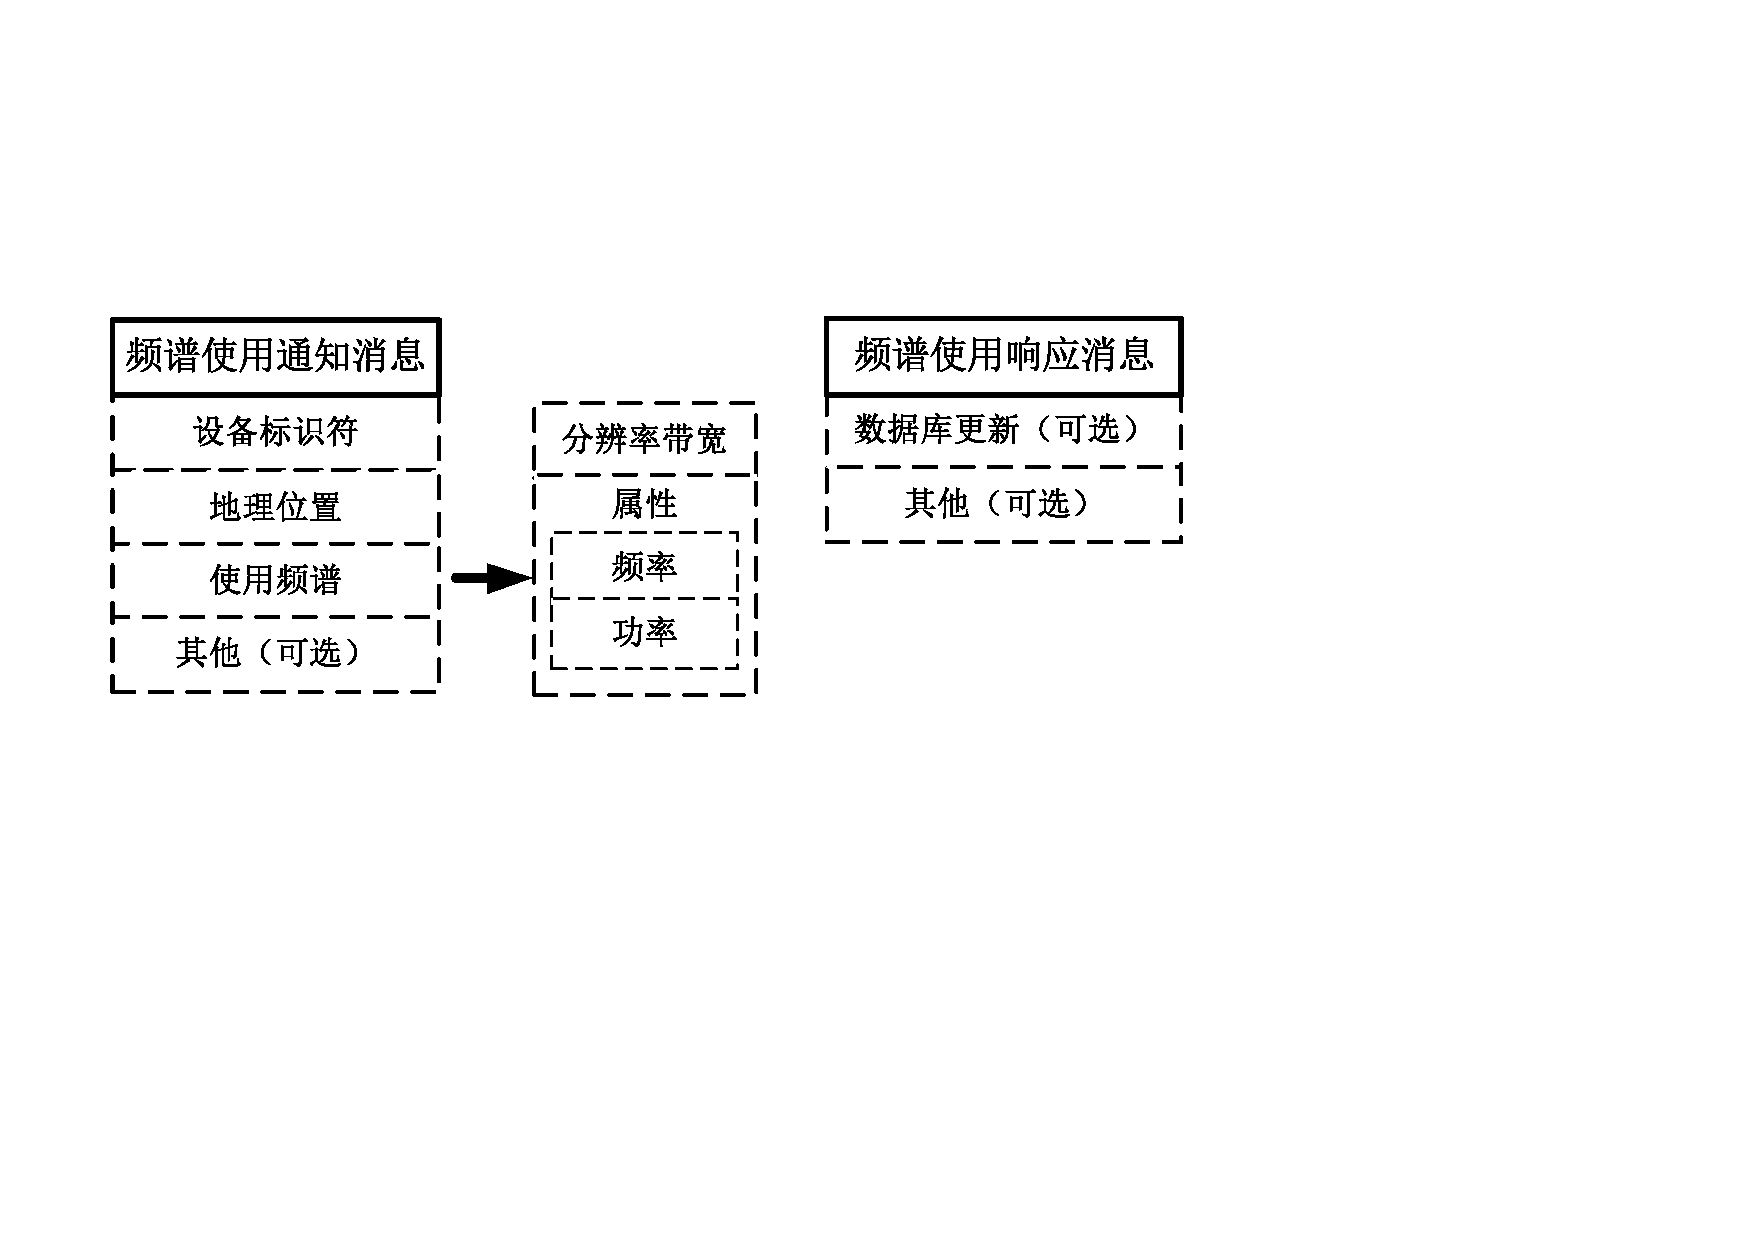
\includegraphics[width=0.65\textwidth]{figures/chap3/standard/query-2}\bicaption[fig:query-2]{频谱通知消息内容}{频谱通知消息内容}{Fig}{Contents of Spectrum Notification}
\end{figure}

频谱使用通知消息是可选功能,但若规则集采用此项功能,则认知用户必须将其使用的频谱和相应传输功率通报给数据库。

\end{enumerate}



HTTPS绑定:PAWS要求使用安全传输层协议(Transport Layer Security,TLS)作为底层的传输机制。TLS提供了认知用户和数据库之间传输消息的完整性和保密性。认知用户必须执行服务器认证,服务器也可以要求用户执行终端设备认证。
PAWS协议中的请求消息应该包含在HTTP POST请求消息中,响应消息应该包含在HTTP响应消息中。



安全方面的考虑:
在PAWS协议的框架下,认知用户和数据库面临如下安全风险:(1)精确度:认知用户收到不准确的可用频谱信息;(2)隐私:未授权者截获通信数据。为规避上述风险,PAWS需要依赖如下措施:

\begin{enumerate}
\item 认知用户必须确定合适的数据库用于查询。
\item 认知用户必须正确连接到合适的数据库。
\item PAWS消息需要保证不被篡改。
\item PAWS消息必须加密。
\end{enumerate}

PAWS允许通过静态指定安全的数据库来保证能够寻找到合适的数据库,采用TLS协议可以规避其他传输层以下的安全风险。此外,为避免精确度造成的风险,数据库需要具备准确计算可用频谱资源的能力,但这不在PAWS协议的考虑范围内。


